\documentclass{book}
\usepackage{geometry}
\usepackage{fancyhdr}
\usepackage{amsmath, amsthm, amssymb}
\usepackage{graphicx}
\usepackage{hyperref}
\graphicspath{ {images/} }

\title{Probability Notes}
\author{Nickson Zhu  \\  \url{nicksonsone@gmail.com}}

\begin{document}
\maketitle
\tableofcontents
\newpage

\chapter{Introduction to Probability}
	\section{Interpretation of Probability}
		\subsection{The Frequency Interpretation of Probability}
			\subsubsection{Definition}
			The probablity that some specific outcome of a process can be intrepreted to 
			mean the relative frequency with which the outcome can be obtained if the 
			process is repeated for a large number of times under similar conditions.  

			\subsubsection{Example}
			Toss coin for 1,000,000 times, number of heads is nearly 500,000, but may 
			not exactly 500,000.

			\subsubsection{Shortcoming} 
			\begin{itemize}
				\item number of tests: how large is enough 
				\item similar conditions: conditions cannot be completely the same, otherwise always same outcome
				\item frequency of outcomes: should approximate theoritical probablity, but no permissible variation
				\item repetition: many important problems have no repetition. For instance, probablity of a aquaintance 
			\end{itemize}

		\subsection{Classical Interpretation \& Subjective Interpretation}
			\subsubsection{Classical}
			Based on equally likely outcome.  Paradox: this concept is based on the 
			probablity we are trying to define.  Example: six-sided dice, equally 1/6.

			\subsubsection{Subjective}
			Based on personal belief and information.  

	\section{Experiments and Events}
		\subsection{Definition}
			\subsubsection{Experiment}
			any process in which the possible outcomes can be identified.  
			\subsubsection{Event}
			a well-define set of possible outcomes of the experiment.  

		\subsection{Explanation}
		Not every set of possible outcomes will be called an event.  The probability 
		of an event will be how likely it is that the outcome is in the event.  

	\section{Set Theory}
		\subsection{Definiton}
			\subsubsection{Set}
			Collection of process outcomes of an experiment.  
			\subsubsection{Empty Set}
			Some events are impossible.  
		
			\subsubsection{Infinite set}
			Infinitely many outcomes.  If countable, there 
			is one-to-one correspondence.  If either finite or countable, 
			a set has at most coutably many items.  

		\subsection{Operations on Sets}
			\subsubsection{Union of Sets}
			If $A_1$, $A_2$, \ldots  are countable collection of events,then 
			$\cup_{i=1}^{\infty}$ is also an event.  But $\cup_{i=1}^{\infty}$ 
			does not necessarily have to be an event.  

			\subsubsection{Overlaps of Evnets}
			Look at the pictures at page \pageref{fig:intersection_1}, 
			if events are not disjoint, their union can be deduced from intersections.  
			\begin{figure}[h]
				\centering
				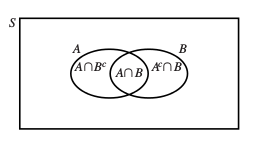
\includegraphics[scale=0.5]{PartitionByTwo}
				\caption{intersection of two events}
				\label{fig:intersection_1}
				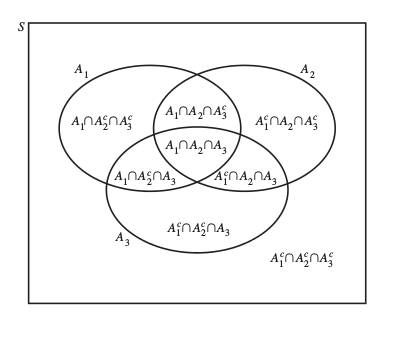
\includegraphics[scale=0.5]{PartitionByThree}
				\caption{intersection of three events}
				\label{fig:intersection_2}
			\end{figure}

			\subsubsection{Useful Theorem}
			\begin{align*}
				A = (A \cap B) \cup (A \cap B^c) \\
				A \cup B = B \cup (A \cap B^c) 
			\end{align*}

	\section{Probability}
		\subsection{Axioms}
		\begin{itemize}	
			\item For every event $A$ ,  $ Pr(A)\geq0 $ 
			\item $Pr(S) = 1$ 
			\item For every infinite sequence of disjoint events
				\[
					Pr\bigg( \bigcup_{i=1}^\infty A_i \bigg) = \sum_{i=1}^\infty Pr(A_i)
				\]
			For finite sequence of disjoint events, equation above still holds
		\end{itemize}
			
		\subsection{Theorems}
		\begin{itemize}
			\item For every two events A and B, $ Pr(A \cap B^c) = Pr(A) - Pr(A \cap B) $.  
			\begin{align*}
				\intertext{The reason is}
				A = (A \cap B) \cup (A \cap B^c)
				\intertext{According to Axiom 3, we have}
				Pr(A) = Pr(A \cap B) + Pr(A \cap B^c)
				\intertext{Therefore}
				Pr(A \cap B) = Pr(A) - Pr(A \cap B^c)
			\end{align*}

		\item For every two events A and B, 
			$ Pr(A \cup B) = Pr(A) + Pr(B) - Pr(A \cap B) $.  
			\begin{align*}
				A \cup B = B \cup (A \cap B^c) \\
				Pr(A \cup B) = Pr(B) + Pr(A \cap B^c)
				\intertext{From theorem above}
				A = (A \cap B) \cup (A \cap B^c) \\
				Pr(A) = Pr(A \cap B) + Pr(A \cap B^c) 
				\intertext{Switch Pr(A) to the right}
				Pr(A \cap B^c) = Pr(A) - Pr(A \cap B) 
				\intertext{Finally}
				Pr(A \cup B) = Pr(A) + Pr(B) - Pr(A \cap 
			\end{align*}

		\item Bonferroni Inequality.  For all events $A_1$,\ldots, $A_n$,	
			\[
				Pr(\bigcup_{i=1}^n A_i) \leq \sum_{i=1}^n Pr(A_i) \text{ and } 
				Pr(\bigcap_{i=1^n A_i}) \leq 1 - \sum_{i=1}^n Pr(A_i^c)
			\]

		\end{itemize}
	\section{Counting Methods}
		\subsection{Multiplication Rule}
		\begin{itemize}
			\item An experiment has $k(k \leq 2)$ parts, that the $i$th part has $n_i$ outcomes
			\item The outcomes of each part is independent of each other 
			\item The total number of possible outcomes is $n_1n_2\cdots n_k$.  
		\end{itemize}

		\subsection{Permutation}
			\subsubsection{Sampling without Replacement}
			Selecting $k$ elements from a set of $n$ at a time without 
			replacement will be a permuation of $n$ elements taken $k$ at 
			a time.  Denoted by $P_{n, k}$, be awared of $0! = 1$
			\[
				P_{n, k} = n(n-1)(n-2)\cdots(n-k+1) 
			\]
			Another form
			\[
				P_{n, k} = n(n-1)(n-2)\cdots(n-k+1)\frac{(n-k)(n-k-1)\cdots1}{(n-k)(n-k-1)\cdots1}
					 = \frac{n!}{(n-k)!}
			\]
			When $ k=n $,
			\[
				P_{n, n} = n! 
			\]

			\subsubsection{Sampling with Replacement}
			Make $k$ selections, all selections have $n$ outcomes.  
			Pick a ball from $n$ for $k$ times, with each time putting the ball back.  
			Suppose the outcome vector is $(x_1, x_2,\ldots,x_k)$, 
			probability assigned to each vector is $\frac{1}{n^k}$



\begin{thebibliography}{9}
	\bibitem{ConcreteMath}
		Ronald L.   Granham, Donald E.  Knuth, and Oren Patashnik,
		\textit{Concrete Mathematics},
		Addison-Wesley, Reading, MA, 1995.
	\end{thebibliography}
\end{document}
